\documentclass[fontset=windows]{article}
\usepackage[margin=1in]{geometry}
\usepackage{ctex}
\usepackage{setspace}
\usepackage{lipsum}
\usepackage{graphicx}
\usepackage{caption}
\usepackage{subcaption}
\usepackage[colorlinks=true,linkcolor=red]{hyperref}

\graphicspath{{figures/}}

\title{\heiti\zihao{2} Common-Source Stage \uppercase\expandafter{\romannumeral2} \& Variants}
\author{\songti zrrraa}
\date{2023.11.19}

\begin{document}
\maketitle
\thispagestyle{empty}

\section*{Simplification}

\begin{figure}[htbp]
    \centering
    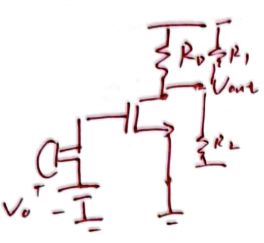
\includegraphics[scale=0.8]{1.jpg}
    \captionsetup{labelformat=empty}
    \caption{}
    \label{1}
\end{figure}

Ignore the Channel-Length Modulation, we can simplify the gain as:

$A_V=-g_m*$(total resistance tied from drain to AC GROUND).

AC GROUND means the point which has a const voltage.

In the picture, we have:

$$A_V=-g_m(R_D||R_1||R_2)$$

\section*{Example}

\begin{figure}[htbp]
    \centering
    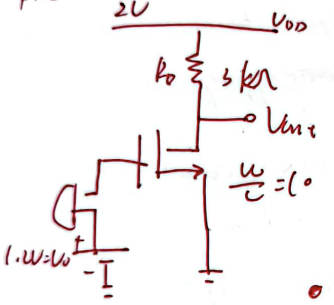
\includegraphics[scale=0.8]{2.jpg}
    \captionsetup{labelformat=empty}
    \caption{}
    \label{2}
\end{figure}

First assume that it's in Sat. zone and then calculate out the $I_D$ and check if the assume is true.

If we want to double the gain, how can we do?

\begin{itemize}
    \item Try doubling $R_D$? $I_D*R_D$ larger, the $V_{DS}$ lower, the MOS will run out fo the saturation zone.
\end{itemize}

We always want an amplifier working in saturation zone because it means larger swing of $I_D$.We want a lower $I_D$ in DC, but higher in AC.

\begin{itemize}
    \item Try increasing $g_m=\sqrt{2\mu C_{ox}\frac{W}{L}I_D}$
\end{itemize}

We shouldn't increase $I_D$, that leads to the same result as increasing $R_D$. 

Then $\frac{W}{L}$? 

It is worth noting that if $\frac{W}{L}$ becomes sufficiently large, $g_m\approx \frac{I_D}{1.5V_T}$. 
$V_T$ here is $\frac{KT}{q}$, 26mV in air. 

\section*{Inclusion of Channel-Length Modulation}

\begin{figure}[htbp]
    \centering
    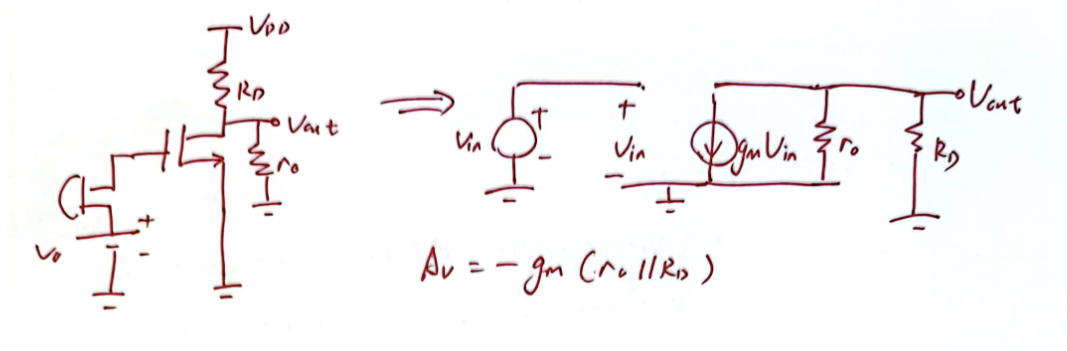
\includegraphics[scale=0.8]{3.jpg}
    \captionsetup{labelformat=empty}
    \caption{Small-Signal Model with Inclusion of Channel-Length Modulation}
    \label{3}
\end{figure}

It's clear that $A_V=-g_m(r_o||R_D)$. 

We want the largest $A_V$, means the largest $R_D$. 
The circuit cannot be open, because we need bias. So, a current source is appropriate. 

\begin{figure}[htbp]
    \centering
    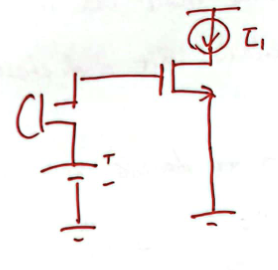
\includegraphics[scale=0.8]{4.jpg}
    \captionsetup{labelformat=empty}
    \caption{}
    \label{4}
\end{figure}

$I_1$ is const \& ideal. We also assume the MOS working in saturation. 

Now $A_V=-g_m*r_o$, we call this intrinsic gain of MOS. It's usually 5~10. 

\section*{Concept of Port Impedance}

\subsection*{input impedance}

\begin{figure}[htbp]
    \centering
    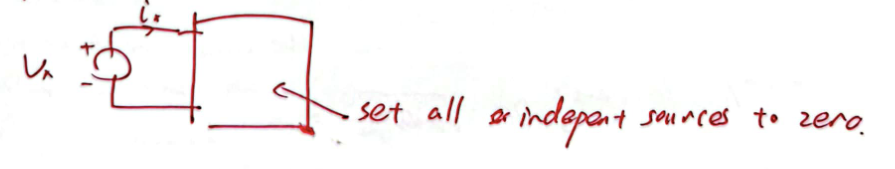
\includegraphics[scale=0.8]{5.jpg}
    \captionsetup{labelformat=empty}
    \caption{}
    \label{5}
\end{figure}

When measuring the input impedance, we set all independent sources to zero. The output port should be open. 

$$R_{in}=\frac{v_x}{i_x}$$

\subsection*{output impedance}

\begin{figure}[htbp]
    \centering
    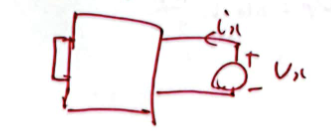
\includegraphics[scale=0.8]{6.jpg}
    \captionsetup{labelformat=empty}
    \caption{}
    \label{6}
\end{figure}

When measuring the output impedance, the input port should be short. 

\section*{Let's build a current source}

\begin{figure}[htbp]
    \centering
    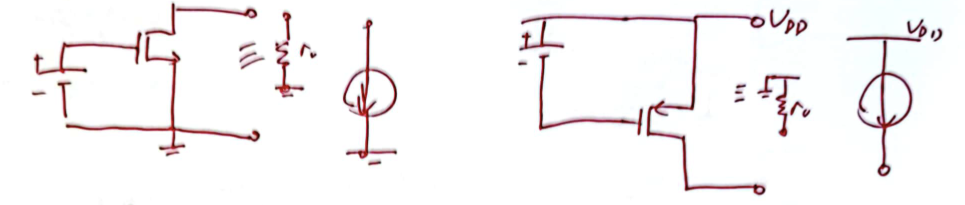
\includegraphics[scale=0.8]{7.jpg}
    \captionsetup{labelformat=empty}
    \caption{}
    \label{7}
\end{figure}

If a MOS is working as a current source, we can refer it as a resistor. (only when $\lambda>0$) 

If $\lambda=0$, we refer it as a open circuit. 

\section*{Common-Source Stage with Current-Source Load}

\begin{figure}[htbp]
    \centering
    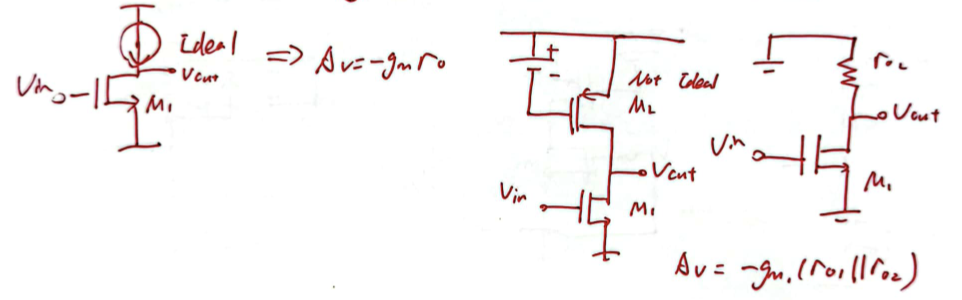
\includegraphics[scale=0.8]{8.jpg}
    \captionsetup{labelformat=empty}
    \caption{}
    \label{8}
\end{figure}

Refer the MOS as a resistor or a open circuit. 

\section*{Common-Source Stage with Diode-Connected Device Load}

\begin{figure}[htbp]
    \centering
    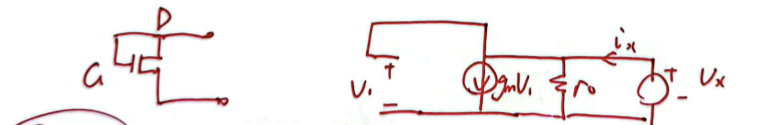
\includegraphics[scale=0.8]{10.jpg}
    \captionsetup{labelformat=empty}
    \caption{}
    \label{9}
\end{figure}

Diode-Connected means the Gate and Drain are short together. 

From the small-signal model we can get the output impedance. 

$$i_x=\frac{v_x}{r_o}+g_mv_1$$

$$v_1=v_x$$

So, 

$$\frac{v_x}{i_x}=r_o||\frac{1}{g_m}$$

Usually, $r_o>>\frac{1}{g_m}$, so the output impedance can be approximately equal to $\frac{1}{g_m}$. 

\begin{figure}[htbp]
    \centering
    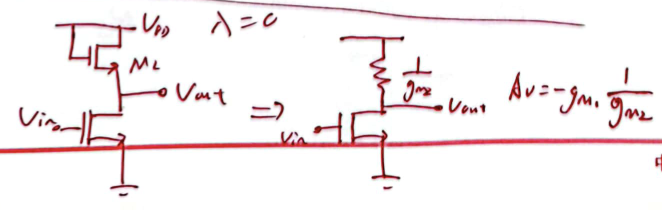
\includegraphics[scale=0.8]{9.jpg}
    \captionsetup{labelformat=empty}
    \caption{}
    \label{10}
\end{figure}

Also we have $A_V=-g_{m1}\frac{1}{g_{m2}}$. 

\section*{Input and Output Impedances}

\subsection*{Resistor Load}

\begin{figure}[htbp]
    \centering
    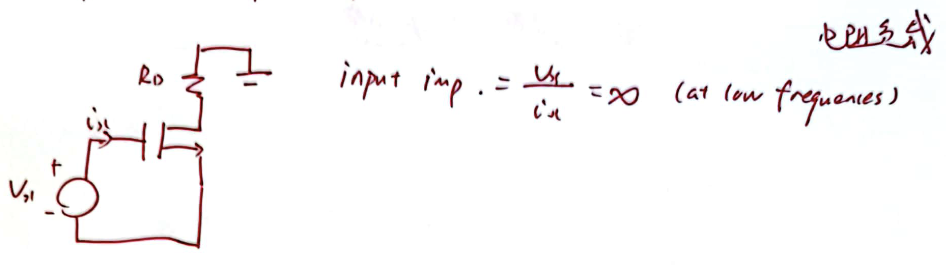
\includegraphics[scale=0.8]{11.jpg}
    \captionsetup{labelformat=empty}
    \caption{}
    \label{11}
\end{figure}

input imp. $=\frac{v_x}{i_x}=\infty$ (at low frequencies)

\begin{figure}[htbp]
    \centering
    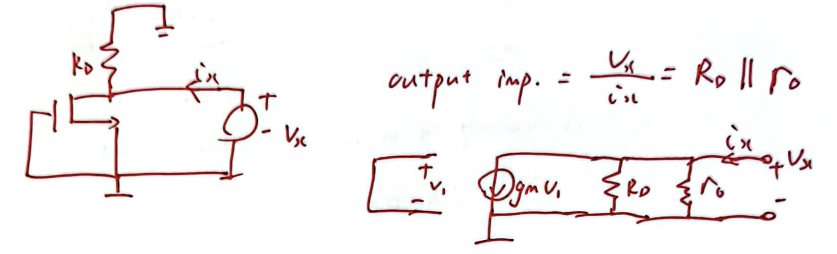
\includegraphics[scale=0.8]{12.jpg}
    \captionsetup{labelformat=empty}
    \caption{}
    \label{12}
\end{figure}

output imp. $=\frac{v_x}{i_x}=R_D||r_o$

\subsection*{Current-Source Load}

\begin{figure}[htbp]
    \centering
    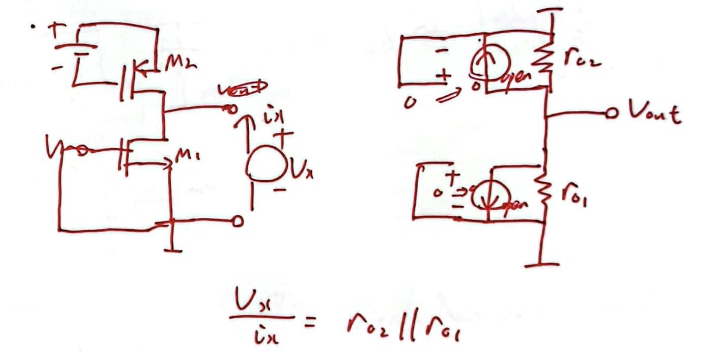
\includegraphics[scale=0.8]{13.jpg}
    \captionsetup{labelformat=empty}
    \caption{}
    \label{13}
\end{figure}

output imp. $\frac{v_x}{i_x}=r_{o2}||r_{o1}$

\subsection*{Diode-Connected Device Load}

\begin{figure}[htbp]
    \centering
    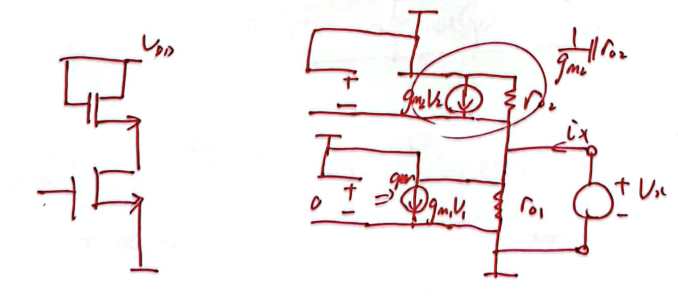
\includegraphics[scale=0.8]{14.jpg}
    \captionsetup{labelformat=empty}
    \caption{}
    \label{14}
\end{figure}

output imp. $=\frac{v_x}{i_x}=\frac{1}{g_m2}||r_{o2}||r_{o1}$

Here $\frac{1}{g_{m2}}$ is dominant. 

\section*{Link}

\href{https://www.bilibili.com/video/BV1FD4y1R7Ah?p=36&vd_source=1d0c07486a3bd3b0adb8ac548bf6453e}{Razavi Electronics Circuits 1: lectrue 36}

\href{https://www.bilibili.com/video/BV1FD4y1R7Ah?p=37&vd_source=1d0c07486a3bd3b0adb8ac548bf6453e}{Razavi Electronics Circuits 1: lectrue 37}
\end{document}